a% Commande exercice bas�e sur une version de Michel Gosse
\newcounter{num}
\renewcommand{\thenum}{\arabic{num}}
\newcommand{\exo}{\addtocounter{num}{1}{\noindent\textbf{Exercice~\thenum~}}}
\newenvironment{exercice}{\exo}{\vskip 0.5cm}

\documentclass[a4paper,10pt,twocolumn]{article}
%\setlength{\textwidth}{18cm}
%\setlength{\oddsidemargin}{0cm}
\usepackage[latin1]{inputenc}
\usepackage[french]{babel}
\usepackage{graphicx}
\usepackage{marvosym}
\title{Devoir Maison 2 - 3$^{\grave{e}me}$}
\date{Pour le 13 novembre 2000}
\begin{document}

\maketitle

\begin{exercice}
  
  Avec 112~\EUR , Joachim a achet� 4 livres et 4 CD. Un CD co�te
  4~\EUR~de plus qu'un livre.

\begin{enumerate}
  \item �crire en fonction de $x$~:
    \begin{enumerate}
      \item le prix d'un CD~;
      \item le prix de 4 CD et de 4 livres.
    \end{enumerate}
  \item �crire un �galit� v�rifi�e par $x$.
  \item Quel est le prix d'un livre. D'un CD~?
\end{enumerate}
\end{exercice}

\begin{exercice}

On donne l'expression~:
$$A=\left(3x+1\right)\left(5x-4\right)-{\left(5x-4\right)}^2$$
\begin{enumerate}
\item Factoriser $A$~;
\item R�soudre l'�quation $(5-2x)(5x-4)=0$.
\end{enumerate}
\end{exercice}


\begin{exercice}

  Un menusier propose � ses clients des portes ayant la forme d'un
  rectangle dont la hauteur est le double de la largeur et qui est
  surmont� d'un demi-disque.  

  La hauteur du rectangle est �gale � $x$. La largeur de la porte
  varie de 70 � 120 cm.
%\begin{center}\includegraphics{dm-3eme-4-2.eps}\end{center}

\begin{center}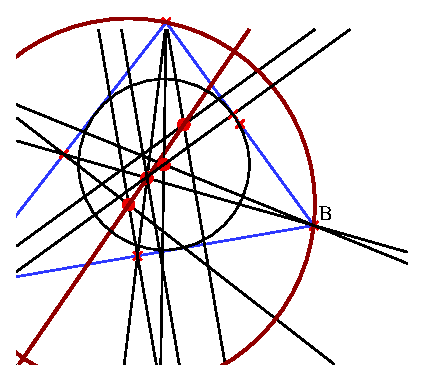
\includegraphics[width=4cm,keepaspectratio=true]{../euler-exporte2.eps}\end{center}


\begin{enumerate}
\item Faire un sch�ma.
\item Calculer la hauteur maximale et la hauteur minimale de la porte.
\item Une cliente voudrait une porte dont la hauteur totale est
  234~cm. Calculer la largeur de cette porte.
\end{enumerate}
\end{exercice}


\begin{exercice}Distance sur la sph�re terrestre

La terre est assimil�e � une boule de rayon 6400~km.
\begin{center}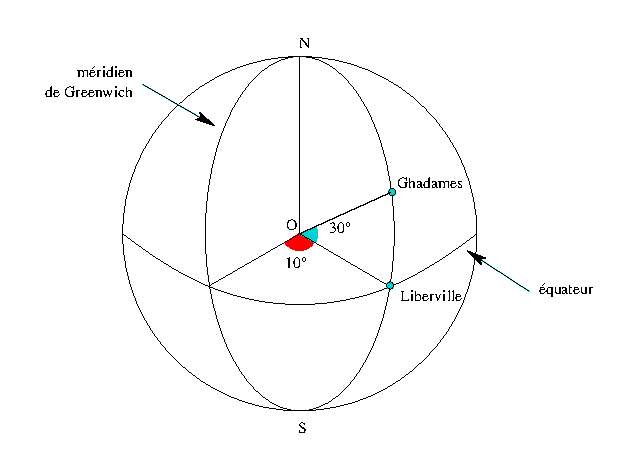
\includegraphics{dm2-1.eps}\end{center}

\begin{enumerate}
\item Calculer la distance Liverville-Ghadames (donner la valeur
  arrondie au km)\footnote{On calculera la longueur d'un arc. Les
    diff�rentes longueurs des arcs d'un cercle donn� sont
    proportionnelles � leurs angles au centre~:
    $\frac{\ell_1}{\alpha_1}=\frac{\ell_2}{\alpha_2}=\ldots$}.
\item Calculer le rayon du parall�le passant par Ghadames (donner la
  valeur arrondie au km).
\end{enumerate}
\end{exercice}
q\end{document}